% test-graphinit.tex -- seule différence voulue entre 2.00 et 2.1
% En 2.00, la macro interne \GR@init@vstyle (rang du style) portait le nom
% de la clé xkeyval vstyle elle-même : après le premier \GraphInit[vstyle=..]
% la clé était détruite jusqu'à la fin du groupe. Les \GraphInit suivants
% étaient ignorés et écrivaient "8Shade" dans le texte.
% En 2.1 chaque \GraphInit[vstyle=...] est pris en compte.
\documentclass{article}
\usepackage{tkz-graph}
\begin{document}
\GraphInit[vstyle=Art]
\GraphInit[vstyle=Shade]  % 2.00 : ignoré, écrit « 8Shade » ; 2.1 : Shade

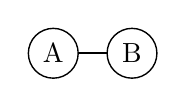
\begin{tikzpicture}
  \Vertex{A}\EA(A){B}\Edge(A)(B)
\end{tikzpicture}

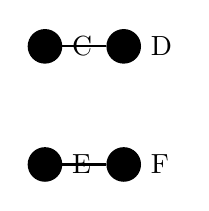
\begin{tikzpicture}
  \GraphInit[vstyle=Classic]
  \Vertex{C}\EA(C){D}\Edge(C)(D)
  \GraphInit[vstyle=Normal] % 2.00 : ignoré
  \Vertex[x=0,y=-1.5]{E}\EA(E){F}\Edge(E)(F)
\end{tikzpicture}
\end{document}
